% \documentclass{book}

\documentclass[12pt]{article}
\usepackage[pdfborder={0 0 0.5 [3 2]}]{hyperref}%
\usepackage[left=1in,right=1in,top=1in,bottom=1in]{geometry}%
\usepackage[shortalphabetic]{amsrefs}%
\usepackage{amsmath}
\usepackage{enumerate}
\usepackage{enumitem}
\usepackage{amssymb}                
\usepackage{amsmath}                
\usepackage{amsfonts}
\usepackage{amsthm}
\usepackage{bbm}
\usepackage[table,xcdraw]{xcolor}
\usepackage{tikz}
\usepackage{float}
\usepackage{booktabs}
\usepackage{svg}
\usepackage{mathtools}
\usepackage{cool}
\usepackage{url}
\usepackage{graphicx,epsfig}
\usepackage{makecell}
\usepackage{array}

\def\noi{\noindent}
\def\T{{\mathbb T}}
\def\R{{\mathbb R}}
\def\N{{\mathbb N}}
\def\C{{\mathbb C}}
\def\Z{{\mathbb Z}}
\def\P{{\mathbb P}}
\def\E{{\mathbb E}}
\def\Q{\mathbb{Q}}
\def\ind{{\mathbb I}}

\begin{document}
\section*{Homework 5}In this problem, we use Fourier spectral methods to solve the 2-D time-dependent incompressible Navier-Stokes equation for the vorticity $\omega$:
\[
\omega_t + (u \omega)_x + (v \omega)_y = \frac{1}{Re} \Delta w
\]
where $Re$ is the Reynolds number and $u$ and $v$ are the velocities in the two spatial directions. The vorticity stream-function $\psi$ is related to the vorticity by $\Delta \psi = \omega$. The velocities $u$ and $v$ are obtained by differentiating the stream-function: $u = \psi_y$ and $v = -\psi_x$. \\

We use both the Fourier collocation method and the Fourier Galerkin method. Time-stepping is done with a fourth-order Runge-Kutta scheme, and we use a CFL number of 0.1 with an end time of $t = 2 \pi$. Periodic boundary conditions are used in the both spatial directions, and the domain of the problem is $[0, 2 \pi] \textrm{x} [0, 2 \pi]$. The Reynolds number for our simulation is 100.  \\

We use two different initial conditions for the problem:
\begin{enumerate}
	\item $u(x, y, 0) = -2 \sin(x) \sin(y) $\\

	The exact solution is known: $u(x, y, t) = -2 \sin(x) \sin(y) e^{- 2 t/{Re}}$ for this initial condition, thus we can do an error analysis. For the error analysis, we look at the discrete $L^2$ error, the continuous $L^2$ error, and the $L^\infty$ error. For the continuous $L^2$ error, we interpolate the solution at the gridpoints using a discrete trigonometric polynomial, then compute the L2 error by Gaussian quadrature. For the $L^\infty$ error, we again interpolate the solution at the gridpoints using a discrete trigonometric polynomial, and find the maximum error over a fine mesh. We will also present the solution as a two-dimentional color contour map.
	\item $u(x, y, 0) = \begin{cases}
			\delta \cos(x) - \frac{1}{\rho} \textrm{sech}^2\left(\frac{y - \pi/2}{\rho}\right) & y < \pi \\
			\delta \cos(x) - \frac{1}{\rho} \textrm{sech}^2\left(\frac{3 \pi/2 - y}{\rho}\right) & y \geq \pi
	\end{cases}$\\

	For this double shear layer problem, we take $\rho = \pi/15$ and $\delta = 0.05$. The exact solution is unknown, so we will present the output as a two-dimentional color contour map.
\end{enumerate}

\subsection*{Fourier Collocation}
For Fourier Collocation, we require that the residual vanish at the grid points. We implemented this method by using Fast Fourier Transform (FFT).

\subsubsection*{First Initial Condition}

For the first initial condition, we used 2, 4, 8, 16, and 32 grid points in each dimension. We did not go higher since machine accuracy was reached almost immediately, and since my computer is not very fast. The error table output of the program is given below.

\begin{figure}[H]
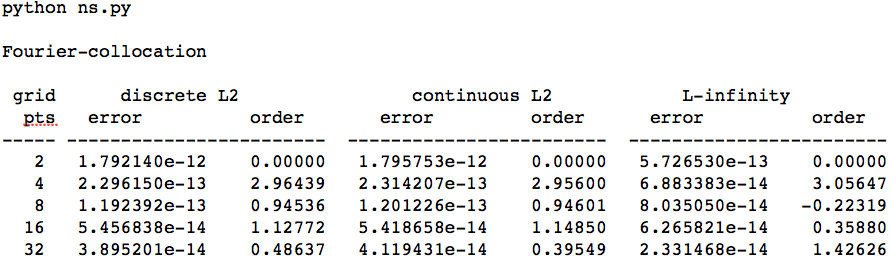
\includegraphics[width=16cm]{images/FourierColloc.png}
\end{figure}

For this method, we also see that machine accuracy is reached even with 2 grid points. This is not surprising, since the initial condition only includes Fourier modes with wavenumber 1, and this should only require 2 Fourier nodes to resolve. In other words, for this initial condition, Fourier spectral methods are exact, and the only error comes from the timestepping scheme. \\

Below we give color contour maps of the output of the scheme for 2 and for 16 grid points in each dimension. We interpolate the solution using discrete trigonometric polynomials before plotting the solution. Note that since the solution essentially consists only of waves with wavenumber 1, the contour maps look almost identical for both 2 and 16 grid points.

\begin{figure}[H]
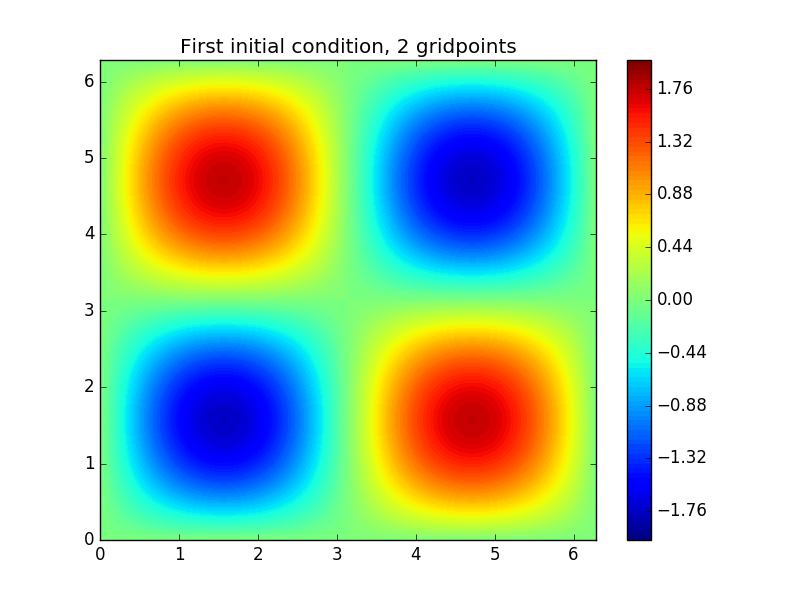
\includegraphics[width=8cm]{images/colloc2.png}
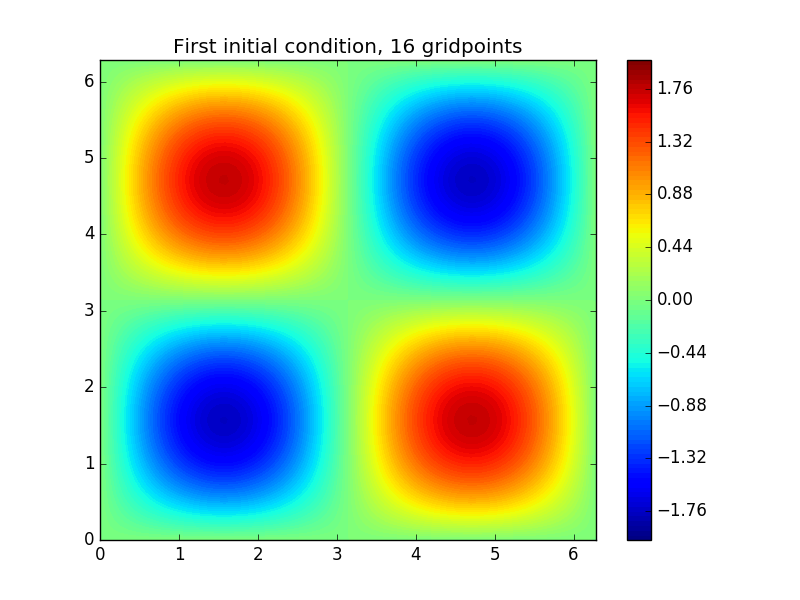
\includegraphics[width=8cm]{images/colloc16.png}
\end{figure}

\subsubsection*{Second Initial Condition}

For the second initial condition (double shear layer), we do not have the exact solution, so we cannot perform an error analysis. We present the output of the scheme after time $t = 2 \pi$ for 16 and 32 grid points in each dimension. Note the development of vorticity rolls. Here we can see that we obtain better resolution with 32 grid points, since there are higher Fourier modes present in the problem, and these higher modes are ignored for smaller numbers of grid points.

\begin{figure}[H]
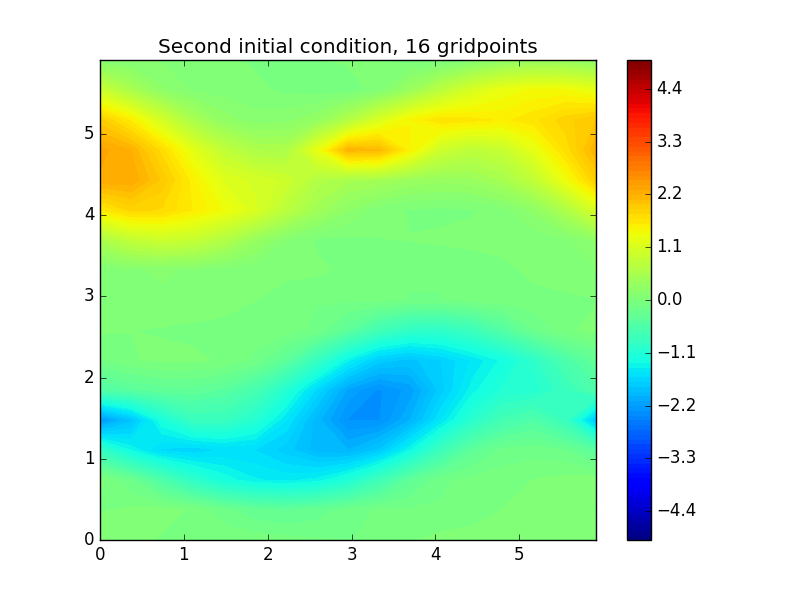
\includegraphics[width=8cm]{images/collocs16.png}
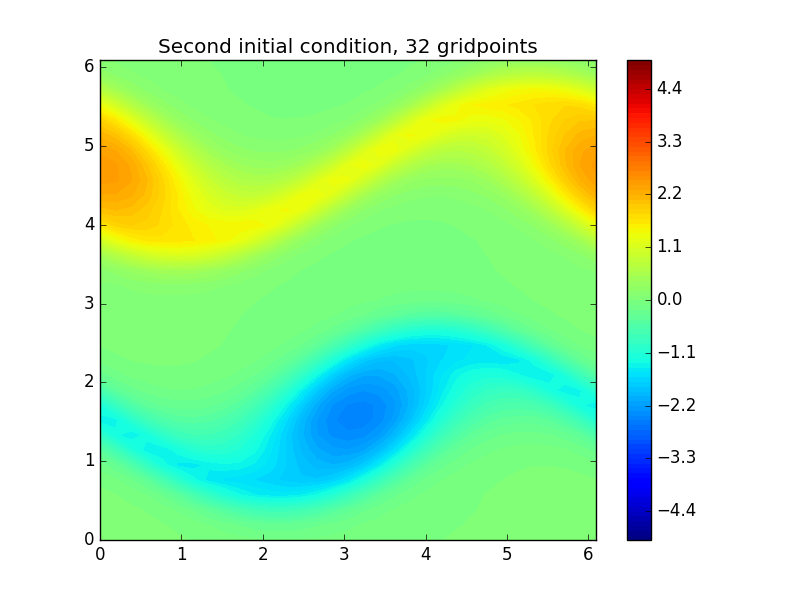
\includegraphics[width=8cm]{images/collocs32.png}
\end{figure}


\subsection*{Fourier Galerkin}
For Fourier-Galerkin with $N$ grid points, we require that the residual be orthogonal to the space $B_N$ of trigonometic polynomials. For this problem, this is equivalent to the following system of ODEs for the Fourier coefficients $b_{np}$, for $-N/2 \leq n, p \leq N/2$:
\begin{align*}
b'_{n,p}(t) &= -\frac{n^2 + p^2}{Re}b_{n,p}(t) - \sum_{|j|,|k|\leq N/2}\frac{-k}{j^2 + k^2}b_{j,k}(t)(n-j)b_{n-j,p-k}(t) \\
&\:\:\:\:- \sum_{|j|,|k|\leq N/2}\frac{j}{j^2 + k^2}b_{j,k}(t)(p-k)b_{n-j,p-k}(t)
\end{align*}

where the two sums on the RHS are discrete convolutions.

\subsubsection*{First Initial Condition}
For the first initial condition, we used 2, 4, 8, 16, and 32 grid points in each dimension. We did not go higher since machine accuracy was reached almost immediately, and since my computer is not very fast. The error table output of the program is given below.

\begin{figure}[H]
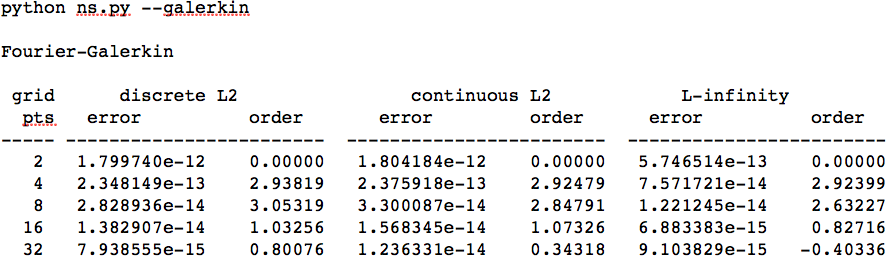
\includegraphics[width=16cm]{images/FourierGalerkin.png}
\end{figure}

For this method, we also see that machine accuracy is reached even with 2 gri dpoints. This is not surprising, since the initial condition only includes Fourier modes with wavenumber 1, and this should only require 2 Fourier nodes to resolve. In other words, for this initial condition, Fourier spectral methods are exact, and the only error comes from the timestepping scheme. \\

Below we give color contour maps of the output of the scheme for 2 and for 16 grid points in each dimension. We again interpolate the solution using discrete trigonometric polynomials before plotting the solution. Note that since the solution essentially consists only of waves with wavenumber 1, the contour maps look almost identical for both 2 and 16 grid points.

\begin{figure}[H]
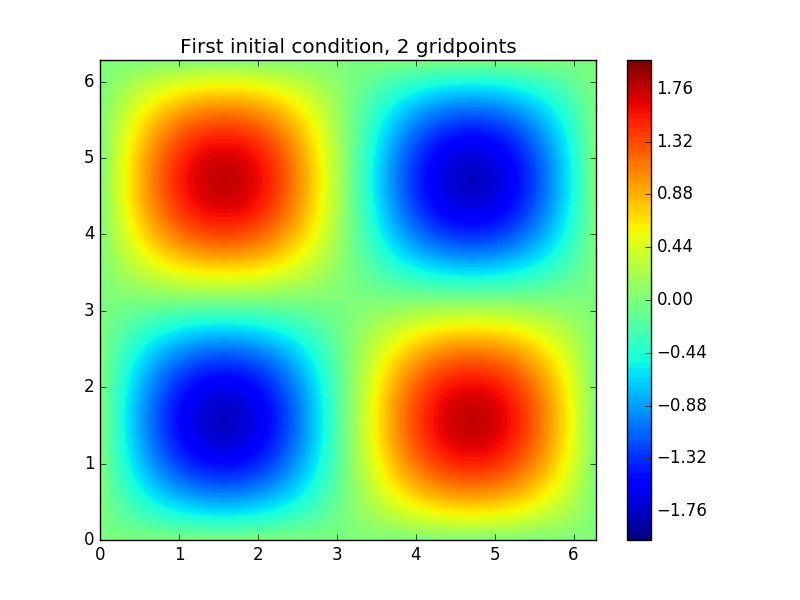
\includegraphics[width=8cm]{images/galerkin2.png}
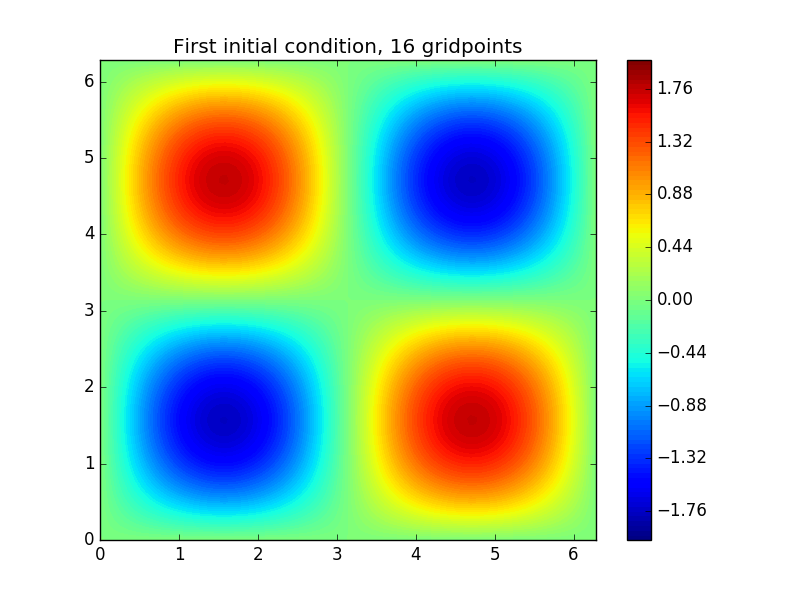
\includegraphics[width=8cm]{images/galerkin16.png}
\end{figure}

\subsubsection*{Second Initial Condition}

For the second initial condition (double shear layer), we do not have the exact solution, so we cannot perform an error analysis. We present the output of the scheme after time $t = 2 \pi$ for 16 and 32 grid points in each dimension. Note the development of vorticity rolls. Here we can see that we obtain better resolution with 32 grid points, since there are higher Fourier modes present in the problem, and these higher modes are ignored for smaller numbers of grid points. Note that the Fouier-Galerkin method output is essentially identical to the Fourier-collocation output.

\begin{figure}[H]
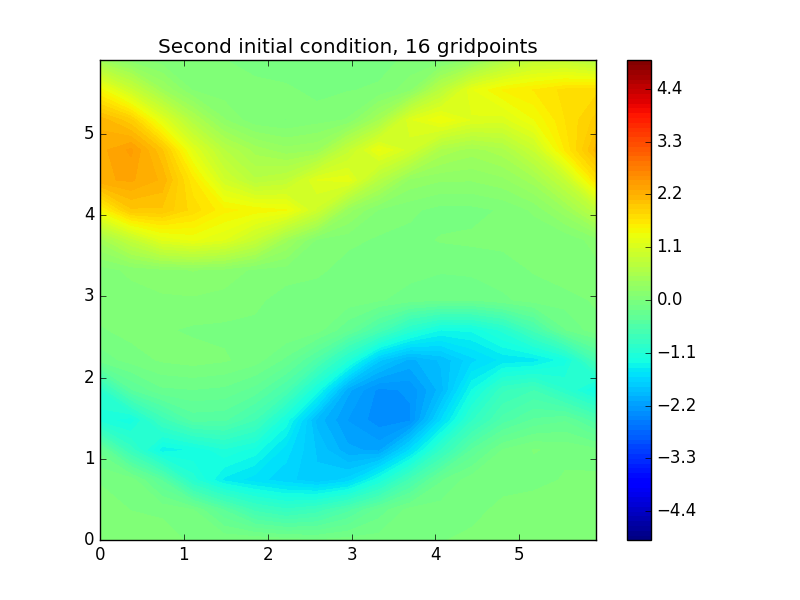
\includegraphics[width=8cm]{images/galerkins16.png}
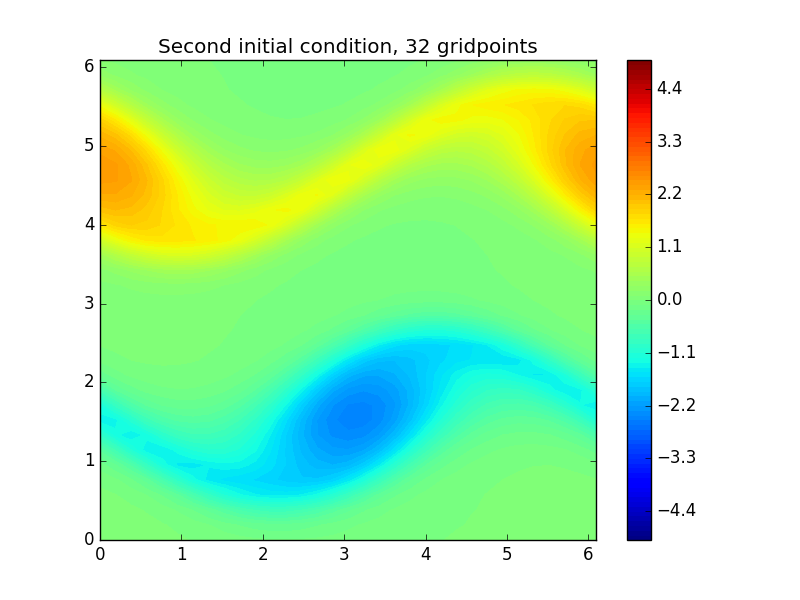
\includegraphics[width=8cm]{images/galerkins32.png}
\end{figure}


\end{document}

